In this chapter, we present experimental results of the LPNN approach. The evaluation is qualitative, since the nature of light probes and their optimal placement is subjective to the user and the needs of the application. We focus mainly on speed in relation to light probe layout given by the tool. We compare performance results to LumiProbes \parencite{Vardis2021}. All experiments were conducted in Unity 6 version 6000.0.38f1, on a system comprising of an NVIDIA RTX2060M GPU, 16GB DDR4 RAM and an Intel i7-9750H CPU, on a Windows 10 Operating System.

\section{Performance}
\label{sec:4_performance}
Since the focus of the thesis was to speed up the placement of light probes in this stage of any 3D application development iteration process, we will focus on the execution time of the tool and also critique the results and their qualitative properties, to make sure the placements are correct. Indeed, as seen in table \ref{table:times}, the LPNN approach speeds up light probe placement by orders of magnitude faster than other approaches, but it may suffer from occasional misplacement; probes that were placed in positions that are not vital, leading to oversampling, which we will show shortly. In experiments where LumiProbes and LPNN were requested to place close to the same amount of light probes in the same scene, LPNN time stayed close to constant, typically up to a few seconds, regardless of the scenario or the amount requested. Results for various amounts of light probes and scenes are presented in table \ref{table:times}. Times are averaged over multiple runs. Units are represented in minutes (m), seconds (s), or milliseconds (ms). Where applicable, we also append the settings used for each tool. For LumiProbes, settings include the grid parameters and the evaluation-point count. All other settings are as follows: Evaluation point placement type is set to Poisson, Decimation type is set to Medium, Decimation directions are averaged, Decimation metric is set to  Chrominance, Minimum LP set is disabled, and Maximum Error is set to 3. For LPNN, settings include the threshold value used for the specific result and the cell size of the 3D grid, in order. Figures for the results are shown in section \ref{sec:4_quality}. Memory requirements for this tool are strictly dependent on the amount of light probes present in the scene, since all information needed by the tool are either already present in Unity and are needed regardless of the presence of the tool, e.g. Global Illumination data, or are stored on the Hard Disk of the system as files with storage sizes dependent on the amount of probes placed before the execution of the tool. File sizes for 150 probes were less than 2KB. Typically, the tool creates files needed for placing the light probes with size-scaling 1KB per approximately 100 probes.

\begin{table}
	\centering
\begin{tabular}{ |c||c|c|c|c|c|  }
	\hline
	\multicolumn{6}{|c|}{Execution time} \\
	\hline
	Method & Scene & Time & P. Count & P. Present (\& Removed) & Settings\\
	\hline
	LumiProbes & Sponza   & 22.443s  & 105 & 34 (75)  & (7,3,5), 128 \\
	\cline{2-6}
	           & Office   & 51.059s  & 144 & 84 (60)  & (12,3,4), 128\\
	           &          & 919.134s & 288 & 182 (106)& (12,3,8), 256\\
	\cline{2-6}
	           & Corridor & 161.151s & 180 & 120 (60) & (20,3,3), 256\\
	           &          & 477.648s & 243 & 147 (96) & (27,3,3), 256\\
	\hline
	\hline
	Ours       & Sponza   & \textbf{5.3ms}  & 90  & 54 (36)   & 0.4, 2.0 \\
			   &          & \textbf{17.8ms} & 400 & 40 (360)  & 0.9, 1.3 \\
	\cline{2-6}
			   & Office   & \textbf{7.8ms}  & 140 & 34 (106)  & 0.758, 1.87 \\
               &          & \textbf{25.2ms} & 832 & 117 (715) & 0.859, 1.10 \\
    \cline{2-6}
    		   & Corridor & \textbf{10.9ms} & 186 & 84 (102)  & 0.549, 1.94 \\
               &          & \textbf{15.7ms} & 246 & 95 (151)  & 0.615, 1.50 \\
               
	\hline
\end{tabular}
\caption{Execution time for LPNN and LumiProbes on a select number of scenes and probe counts. \textit{P. count} represents the total amount of probes in the scene, before simplification. \textit{P. Present} depict the final amount of probes after running the tools. The number in parenthesis is the amount of probes removed by the tool, in respect to the settings. Fastest times are shown in \textbf{bold}.}
\label{table:times}
\end{table}

\section{Quality}
\label{sec:4_quality}
The tools were tested on the aforementioned edited Sponza scene \parencite{Sponza2017}, Corridor scene \parencite{Corridor2021} and Office scene \parencite{Office2021}. We will present the qualitative results. As we will see shortly, LPNN correctly places light probes in areas of high variance.

\begin{figure}[h]
	\centering
	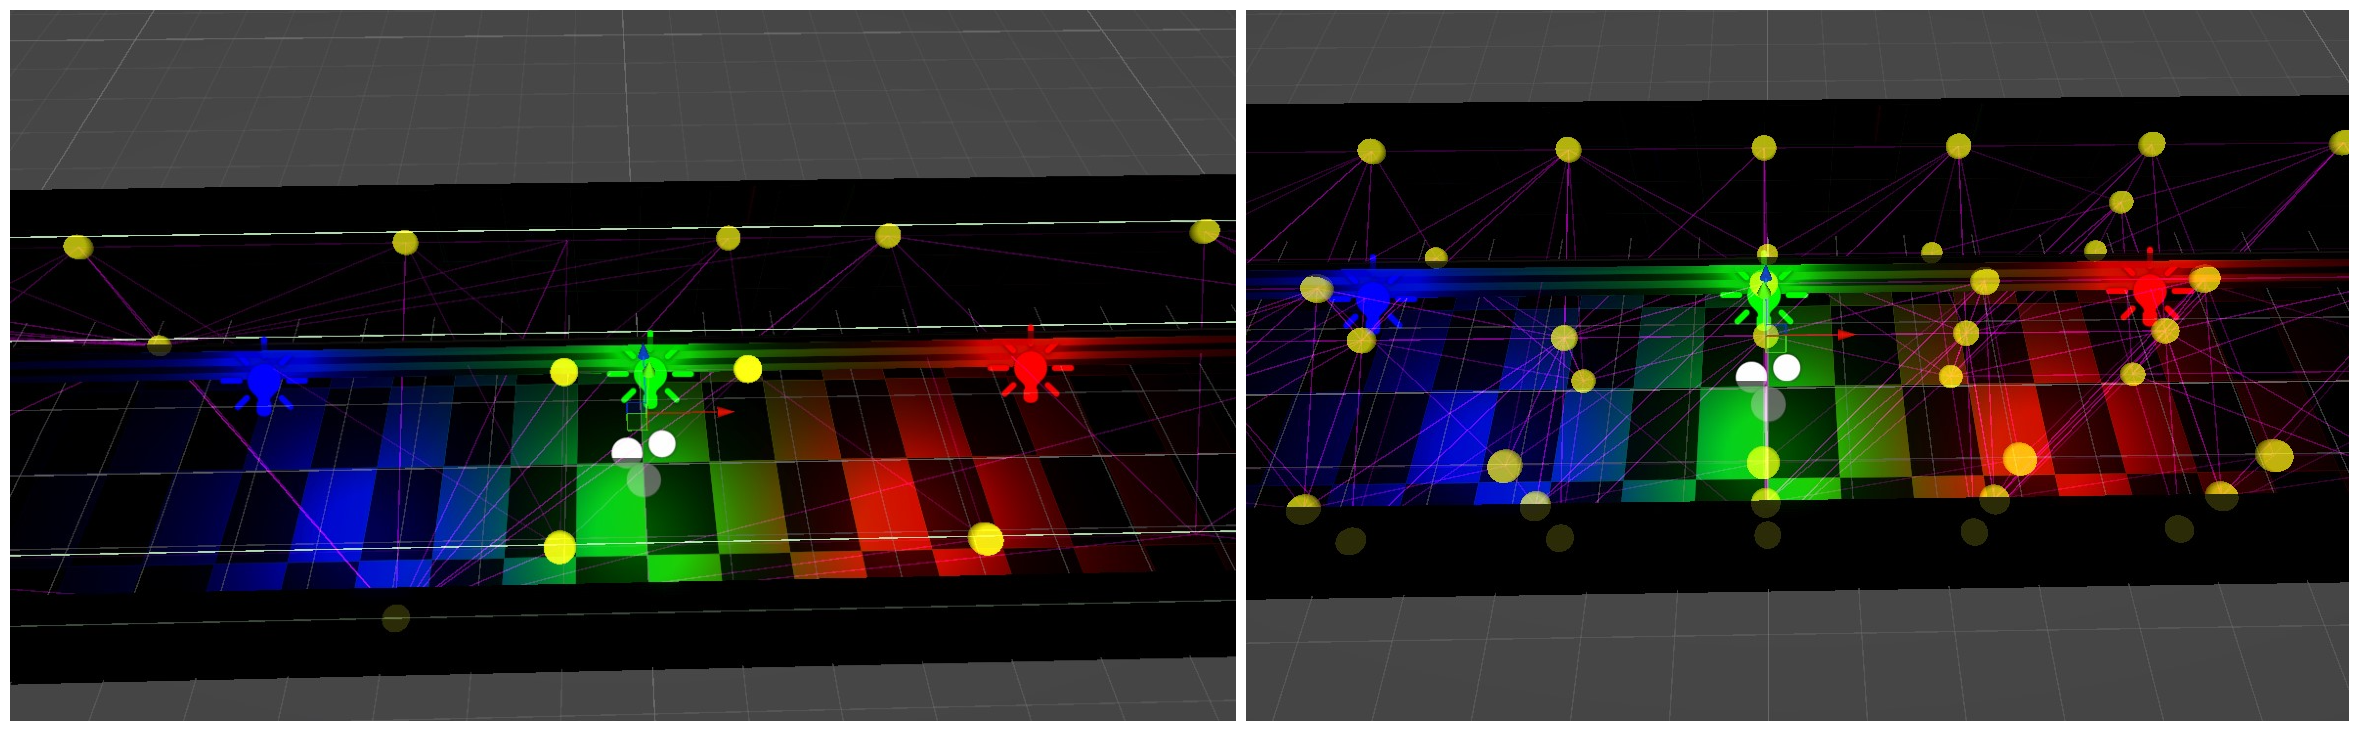
\includegraphics[scale=0.18]{Graphics/results/concats/comparison1.png}
	\caption{A 3D Scene showing a comparison of light probe placement in a \textbf{high} color-variance scenario, between LPNN (left) and LumiProbes (right) with settings 0.549, 1.94 and (27,3,3), 256 respectively, in the Corridor scene.}
	\label{fig:comp1}
\end{figure}

As shown in figure \ref{fig:comp1}, we can clearly see that the LPNN tool has correctly placed light probes between the blue and green light sources, as well as between the green and red light sources, locations with great variance in Chrominance, It has additionally kept the amount of probes at a minimum, only placing one probe at each location mentioned. This result is close to optimal placement, since the distance between the light sources is only 4 units, making additional probes unnecessary in most scenarios. It should be noted that the tool did correctly place probes on the edges of the bounds, seen as light-green colored lines. This ensures that any dynamic object that moves outside the bounds set by the user continues to have some light-probes information for its illumination. 

Furthermore, in figure \ref{fig:comp2} we can see a similar result. The light probe between the two white light sources is vital. The areas left and right from the two light sources have light probes only in the dark areas, making the light transition when a dynamic object moves within this section of the scene smooth. Additionally, the light sources are next to an opaque wall, meaning no light present on the other side of the wall. Therefore, the model decided that placing light probes is only important on the edges of the wall, which is what we see in the example. It is important to note that on the left side of the corridor, as seen in the left image of figure \ref{fig:comp2}, the model has placed a great amount of light probes, even though there is low light variance since that section of the scene is not illuminated. Additionally, as seen in figure \ref{fig:comp3}, the model suffers from under-sampling in certain scenarios; placing fewer light probes than necessary, resulting in partially incorrect lighting. However, this can be resolved in two immediate ways; the user can execute the tool again with different parameters, as seen in figure \ref{fig:comp4}, or the user can manually place a small number of light probes in locations they deem vital. The tool has placed only 2 light probes on the lower section of the scene, resulting in elongated tetrahedrons and incorrect lighting for dynamic objects placed low. Additionally, the light probes placed on the dark side of the wall in figure \ref{fig:comp3} require one more row of light probes placed next to the wall, making any object inside that section of the scene completely dark due to the lack of light in that section. With the settings present in figures \ref{fig:comp1}, \ref{fig:comp2}, and \ref{fig:comp3}, the tool doesn't have enough light probes in the desired locations to correct this issue. This can be fixed by decreasing the cell size parameter.

\begin{figure}[h]
	\centering
	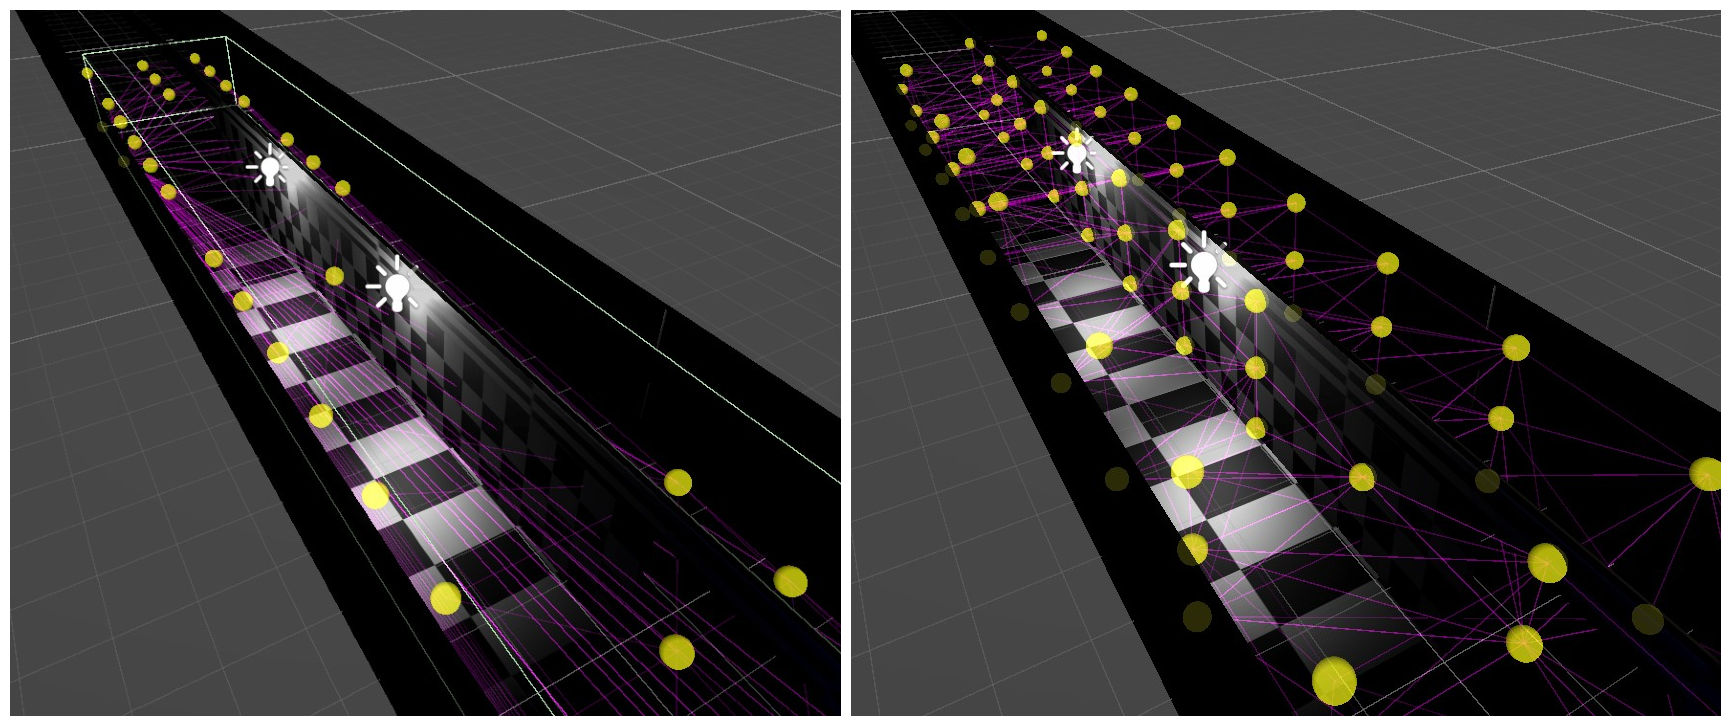
\includegraphics[scale=0.25]{Graphics/results/concats/comparison2.png}
	\caption{A 3D Scene showing a comparison of light probe placement in a \textbf{low} color-variance scenario, but \textbf{high} luminance variance, between LPNN (left) and LumiProbes (right) with settings 0.615, 1.5 and (27,3,3), 256 respectively, in the Corridor scene.}
	\label{fig:comp2}
\end{figure}

\begin{figure}[h]
	\centering
	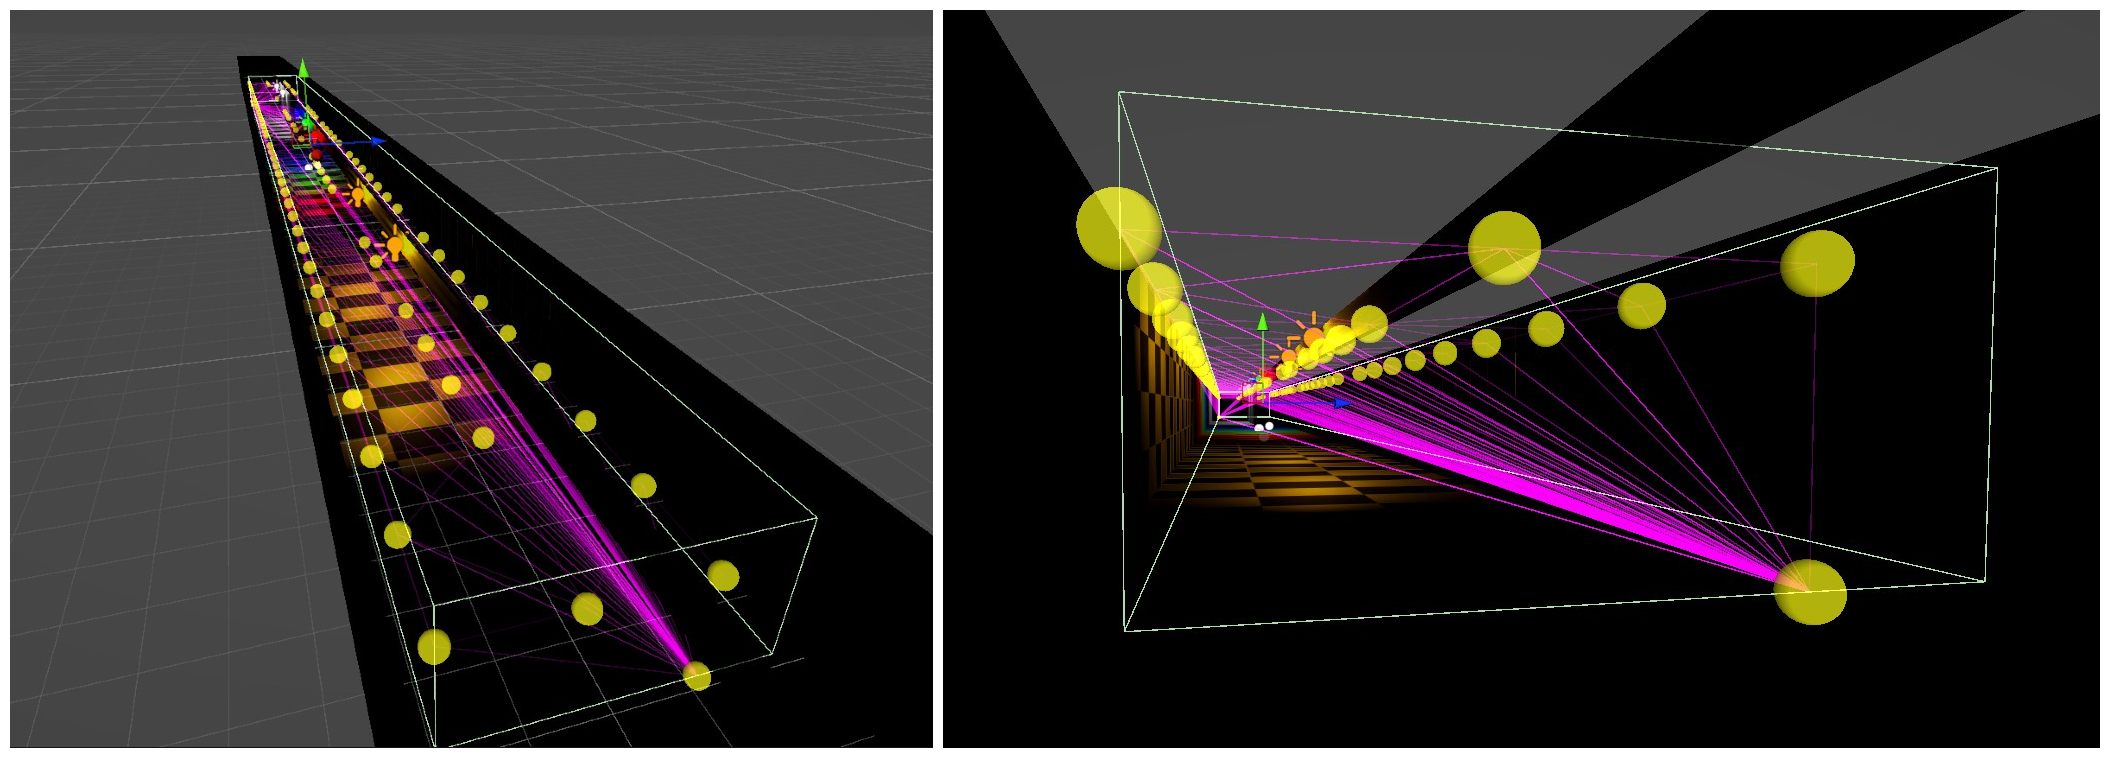
\includegraphics[scale=0.207]{Graphics/results/concats/comparison3.png}
	\caption{A 3D Scene showing under-sampling of light probe placement in the Corridor scene. The example was captured with LPNN with settings 0.615, 1.5.}
	\label{fig:comp3}
\end{figure}

With different settings, as seen in figure \ref{fig:comp4}, we can resolve the under-sampling issue from figure \ref{fig:comp3}. By increasing the cell size but reducing the threshold, the tool has placed more probes on the lower section of the scene, from just 2 to 8, leading to better results overall.

\begin{figure}[h]
	\centering
	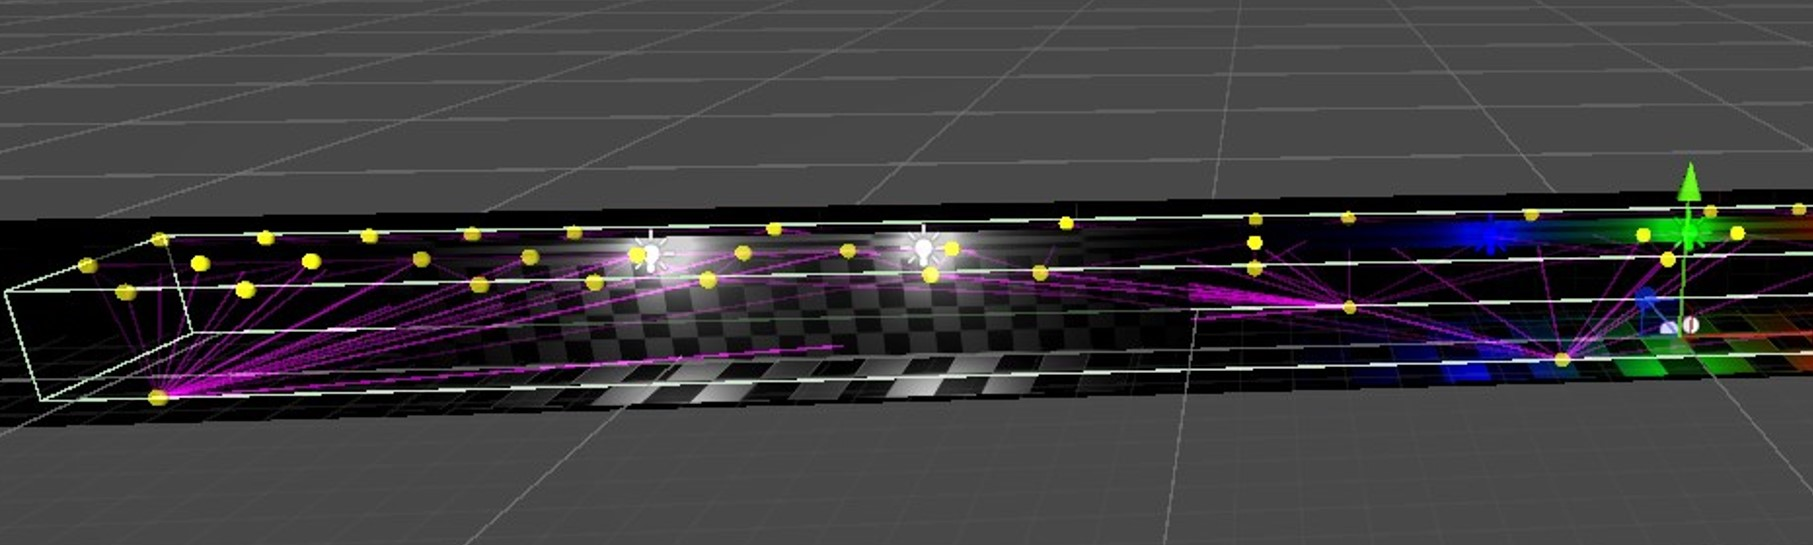
\includegraphics[scale=0.32]{Graphics/results/corridor_0.549_1.94_E2.jpg}
	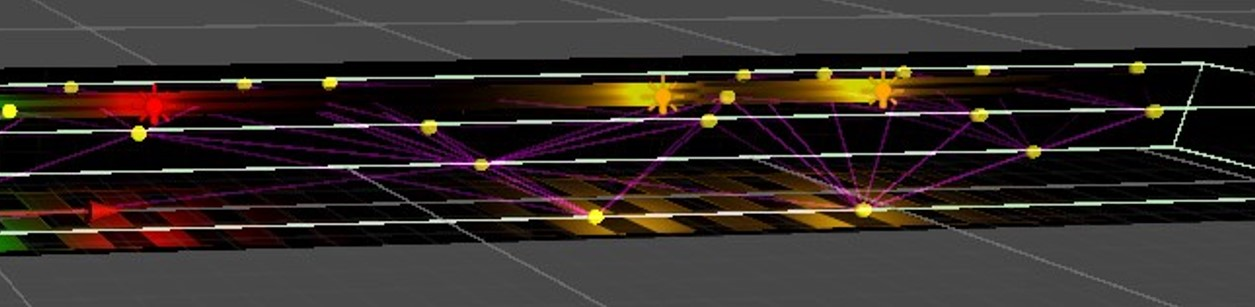
\includegraphics[scale=0.4623]{Graphics/results/corridor_0.549_1.94_E3.jpg}
	\caption{A 3D Scene showing improved light probe placement in the Corridor scene. The example was captured with LPNN with settings 0.549, 1.94.}
	\label{fig:comp4}
\end{figure}



